\chapter{Plataformas de desarrollo y herramientas utilizadas}
\label{cap:capitulo3}

En este apartado se hablará de los recursos ingenieriles empleados para hacer posible el proyecto.

\section{Lenguajes de programación}
\label{sec:lenguajes_programacion}

\subsection{Python}
\label{subsec:python}

A día de hoy, es considerado el lenguaje de programación más popular \footnote[1]{\url{https://www.tiobe.com/tiobe-index/}}. Se ideó en 1991 por Guido van Rossum y se desarrolló en la Python Software Foundation \footnote[2]{\url{https://www.geeksforgeeks.org/history-of-python/}}. Es interpretado, es decir, usa un programa que traduce las líneas de código para la máquina en tiempo de ejecución (lo cual lo hace más intuitivo pero menos eficiente). Además, permite la programación orientada a objetos en alto nivel, lo que ofrece gran dinamismo a la hora de usarlo \footnote[3]{\url{https://www.python.org/doc/essays/blurb/} \url{https://www.educative.io/blog/compiled-vs-interpreted-language}}.\\

Debido a su amplia popularidad, podemos acceder a una gran variedad de módulos y utilidades desarrollados por la comunidad, los cuales se integran perfectamente en la resolución de nuestro problema.\\

En nuestro caso, python se usó para el crear la mayor parte del código empleado, es decir, para desarrollar interfaces gráficas, para trabajar con el middleware robótico \ac{ROS} (detallado posteriormente) y para el desarrollo de los diversos algoritmos. Todo ello haciendo uso del módulo \textbf{numpy}, el cual nos permite realizar operaciones matemáticas y trabajar con vectores de forma rápida y eficiente; así cómo del módulo \textbf{matplotlib}, del cual hablaremos más adelante.\\

\begin{code}[H]
\begin{lstlisting}[language=Python]
#! /usr/bin/env python

if __name__ == "__main__":
	C = 3.0 * (10 ** 8)
	freq = 5 * (10 ** 9)
	lmbda = C / freq
\end{lstlisting}
\caption[Obtención del parámetro lambda en función de una frecuencia (en este caso 5G)]{Obtención del parámetro $\lambda$ en función de una frecuencia (en este caso 5G)}
\label{cod:helloworld_python}
\end{code}

\subsection{C++}
\label{subsec:cplusplus}

También bastante popular, se encuentra el lenguaje de programación creado por Bjarne Stroustrup, en los laboratorios Bell en 1971. En este caso es compilado, lo que implica la traducción y enlazado previo a la ejecución. De corte más eficiente que Python, también permite la programación orientada a objetos. Se sitúa a medio camino entre un lenguaje de alto nivel y uno de bajo nivel \footnote[4]{\url{https://www.geeksforgeeks.org/history-of-c/}}.\\

El uso designado en este proyecto para este lenguaje fue para poder trabajar con mapas de calor, mediante la biblioteca de \emph{Anybotics} de grid maps\footnote[5]{\url{https://github.com/ANYbotics/grid_map}}.

\begin{code}[H]
\begin{lstlisting}[language=C++]
#include <iostream>

int main(int argc, char ** argv) {
    std::cout << "Hello World!" << std::endl;
    return 0;
}
\end{lstlisting}
\caption[Hello world en C++]{\emph{Hello world} en C++}
\label{cod:helloworld_cplusplus}
\end{code}

\section{\ac{ROS}}
\label{sec:ros}

Si se habla de robótica, se habla de \ac{ROS}, ya que es el framework para el desarrollo de soluciones de este ámbito, pero, ¿qué es exactamente \ac{ROS}?.\\

Se trata de un \emph{middleware}, es decir, una infraestructura software situada entre el sistema operativo y el desarrollador, que incluye una serie de módulos y funcionalidades enfocadas al desarrollo de aplicaciones robóticas \footnote[6]{\url{https://www.ibm.com/topics/middleware} \url{https://www.ros.org/}}. La idea detrás, busca estandarizar soluciones que no dependan de los drivers de cada sensor y actuador presentes. De forma general, se trata de una arquitectura basada en el paradigma de publicador-suscriptor, donde una serie de nodos se comunican entre sí, transmitiendo mensajes propios, a través de canales compartidos llamados \emph{topics}, esto es, un nodo suscriptor se suscribirá a un determinado topic, que permita la transmisión de un tipo de mensaje concreto, quedando en espera de que un nodo pulicador, envíe mensajes de este tipo a ese topic. Todo se gestiona de manera centralizada, es decir, existe un master que se encarga de gestionar el registro de todos los nodos a los topics pertinentes.\\

Concretamente, se usa para desarrollar todos los algoritmos robóticos y para realizar las comunicaciones necesarias en la simulación del dron.\\

Entre las herramientas usadas en este proyecto, se encuentran las siguientes.

\begin{figure} [H]
	\begin{center}
	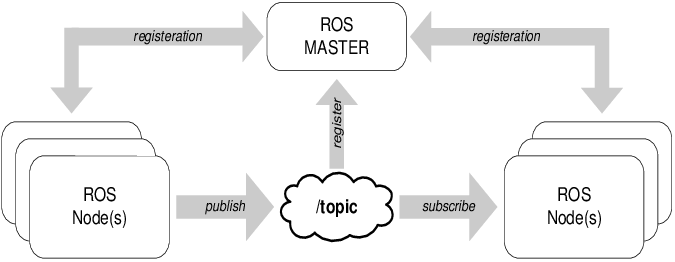
\includegraphics[height=3.25cm]{imagenes/cap3/1_ros_esquema.png}
	\end{center}
	\caption[Esquema de comunicaciones en ROS]{Esquema comunicaciones en ROS}
	\label{fig:ros}
\end{figure}

\subsection{Rviz}
\label{subsec:rviz}

Por el otro lado, se encuentra \emph{rviz}, que es un visualizador 3D diseñado para la depuración de aplicaciones \ac{ROS} \footnote[7]{\url{https://github.com/ros-visualization/rviz}}.\\

En nuestro caso, nos permite ver como se dispersa la señal \ac{RF}, que trayectoria y orientación sigue el dron, que efecto tiene sobre la señal la presencia de obstáculos, y otras tantas opciones.\\

\begin{figure} [H]
	\begin{center}
	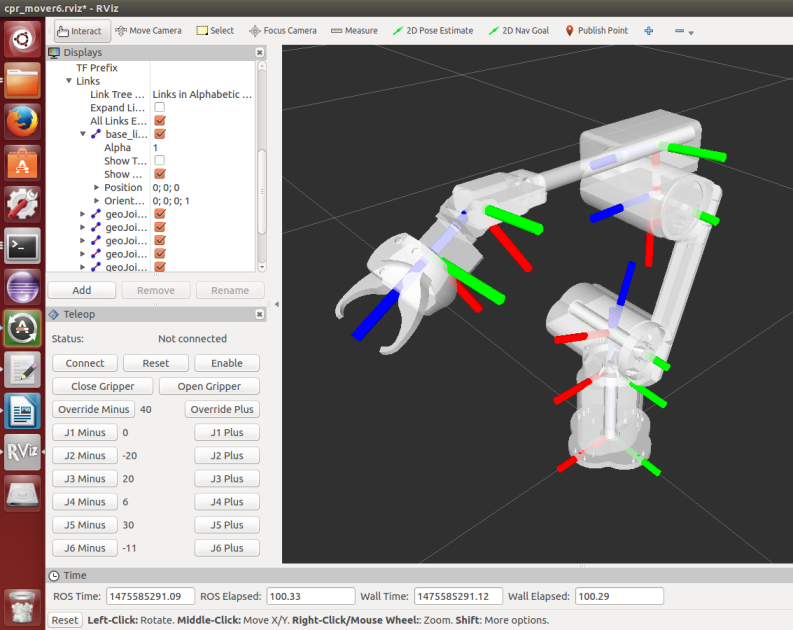
\includegraphics[height=5cm]{imagenes/cap3/3_rviz_example.png}
	\end{center}
	\caption[Ejemplo de uso de Rviz]{Ejemplo de uso de Rviz}
	\label{fig:rviz}
\end{figure}

\section{Gazebo 11}
\label{sec:gazebo}

Se trata del simulador sobre el cual se desarrolla el proyecto. Concretamente consta de un conjunto de módulos optimizados para desarrollar aplicaciones robóticas, ampliamente compatible con \ac{ROS}. Además, posee un motor de físicas basado en ODE, lo que permite simular con precisión el funcionamiento de un dron \footnote[8]{\url{https://gazebosim.org/about}}.\\

Esta herramienta, nos permite visualizar en directo, el comportamiento del dispositivo frente a los diversos escenarios que se planteen.

\begin{figure} [H]
	\begin{center}
	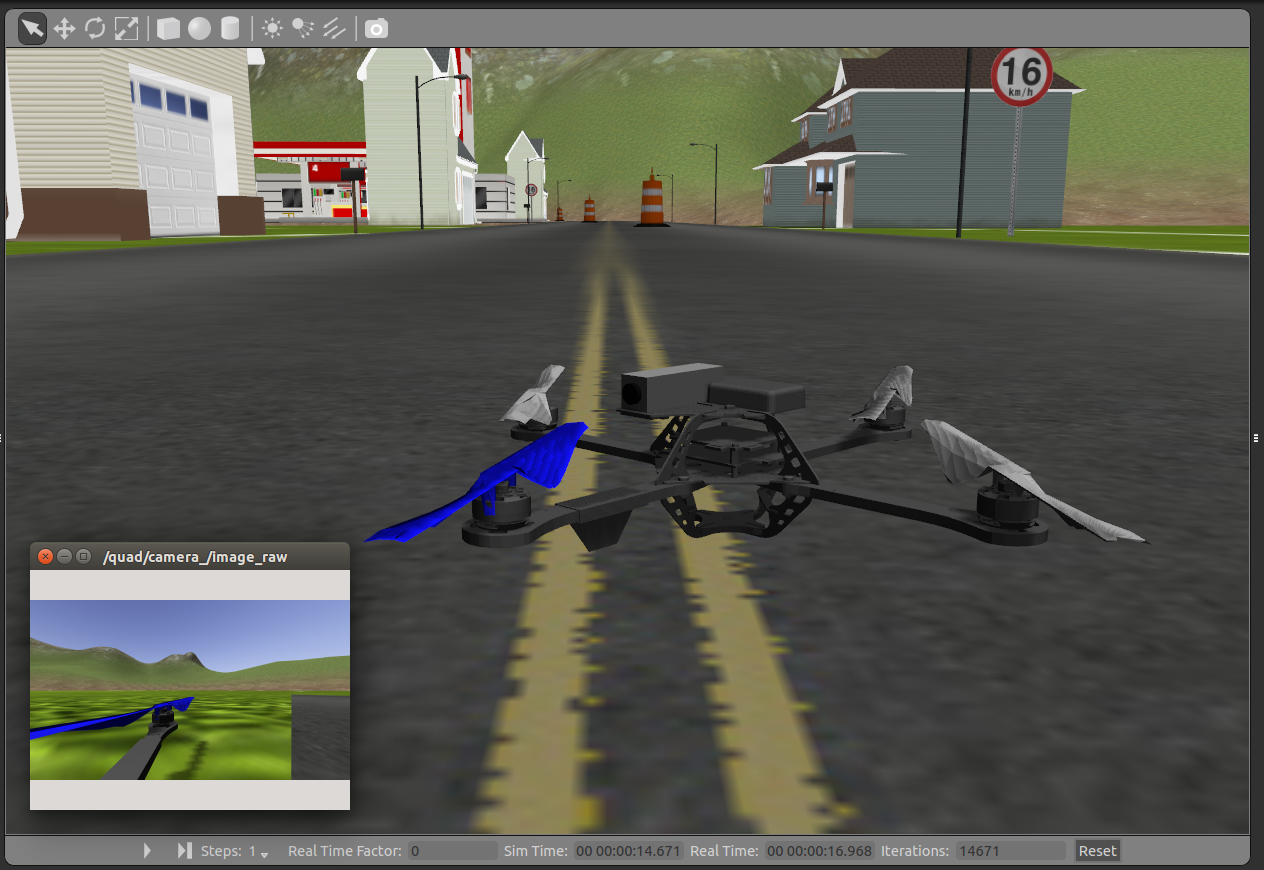
\includegraphics[height=5cm]{imagenes/cap3/2_gazebo_drone.png}
	\end{center}
	\caption[Simulación dron en Gazebo]{Simulación dron en Gazebo}
	\label{fig:gazebo}
\end{figure}

\section{Plataformas de programación}
\label{sec:plataformas_de_programacion}

\subsection{Visual Studio Code}
\label{subsec:visual_studio_code}

Entre las plataformas usadas para programar, \emph{Visual Studio Code}, o mejor conocido como \emph{VS code}, es un editor de código ligero, funcional tanto en Linux, Windows y macOS \footnote[9]{\url{https://code.visualstudio.com/docs}}.\\

Su principal ventaja, es que es altamente personalizable a el tipo de desarrollo software que se desee realizar. Todo ello a través de las múltiples extensiones que ofrece, así como la conexión directa y fluida con plataformas como Github, que se detallarán a continuación.\\

\begin{figure} [H]
	\begin{center}
	
\includegraphics[height=3cm]{imagenes/cap3/4_vscode_logo.png}
	\end{center}
	\caption[VS Code logo]{VS Code logo}
	\label{fig:vscode}
\end{figure}

\subsection{Github}
\label{subsec:github}

Github nace de la herramienta \textbf{git}, creada por Linus Torvalds (desarrollador de Linux), que es un sistema de control de versiones, que funciona a grandes rasgos a través de repositorios (o lugares donde se almacenan los sistemas de versiones de forma local), y commits (que permiten actualizar la version del código almacenado del repositorio) \footnote[10]{\url{https://www.howtogeek.com/180167/htg-explains-what-is-github-and-what-do-geeks-use-it-for/}}.\\

De este modo, Github consiste en trasladar la idea de tener repositorios locales, para distribuirlos en una plataforma online, donde además se permita el desarrollo de aplicaciones de manera colaborativa.\\

Por ello, el papel que toma en este proyecto es de vital importancia, ya que asegura un seguimiento y una seguridad, de cara a tener copias de seguridad, donde todo el que desee puede acceder a ver en que punto se encuentra el \ac{TFG} pueda hacerlo.\\

\section{Módulos}
\label{sec:modulos}

\subsection{OpenCV}
\label{subsec:opencv}

Es una biblioteca software de python, enfocada a visión artificial, y que además dispone de otras funcionalidades útiles para el desarrollo \footnote[11]{\url{https://opencv.org/about/}}.\\

Por tanto, el uso designado en este proyecto es el de implementar interfaces gráficas sencillas, sobre las que interactuar dinámicamente con el dron, a través de barras de acción y botones.

\begin{figure} [H]
	\begin{center}
	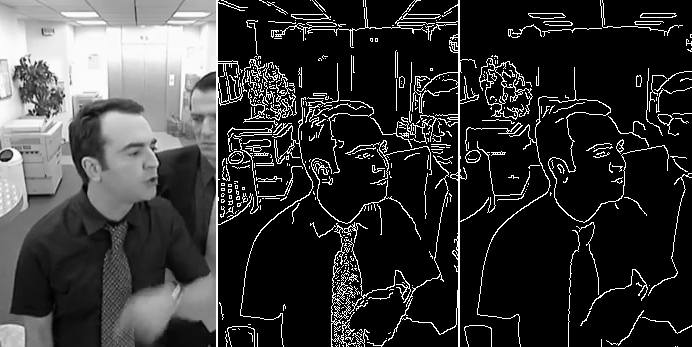
\includegraphics[height=5cm]{imagenes/cap3/5_opencv_example.png}
	\end{center}
	\caption[Interfaz gráfica usando OpenCV]{Interfaz gráfica usando OpenCV}
	\label{fig:opencv}
\end{figure}

\subsection{Matplotlib}
\label{subsec:matplotlib}

Presentada por John Hunter en 2002, se usó como alternativa para el desarrollo de interfaces gráficas. La gran diferencia radica en que está diseñada para trabajar con estructuras numéricas del tipo array (muy compatible con Numpy \footnote[12]{\url{https://numpy.org/about/}}), lo que permite ofrecer una gran visualización y una interfaz responsiva \footnote[13]{\url{https://www.geeksforgeeks.org/python-introduction-matplotlib/}}.\\

Concretamente en este proyecto se usa para desarrollar implementar mapas de calor (que en definitiva son estructuras numéricas del tipo array) dentro de una interfaz gráfica, para simular el comportamiento de una señal \ac{RF}, permitiendo modificar los parámetros de la ecuación en tiempo real.

\begin{figure} [H]
	\begin{center}
	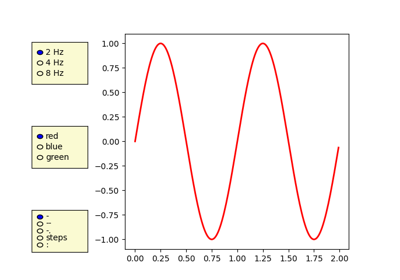
\includegraphics[height=7cm]{imagenes/cap3/6_matplotlib_app.png}
	\end{center}
	\caption[Representación de un mapa de calor usando matplotlib]{Representación de un mapa de calor usando matplotlib}
	\label{fig:matplotlib}
\end{figure}

\subsection{PX4 autopilot}
\label{subsec:px4}

Es la capa de software que permite hacer funcionar las aeronaves con sus componentes, esto es a través del controlador de vuelo, que a efectos prácticos se trata del cerebro del sistema, es decir, interconecta los sensores y actuadores, permitiendo comandar diversas acciones \footnote[14]{\url{https://www.droneblog.com/drone-controller/} \url{https://docs.px4.io/main/en/}}.\\

Este sistema, usa un conocido protocolo de comunicaciones llamado \textbf{MAVLink}, que se encarga de gestionar la comunicación entre el controlador de vuelo y la \ac{GCS}. En nuestro caso, y como queremos desarrollar aplicaciones mediante \ac{ROS}, debemos añadir una capa más, que se encarga de traducir los mensajes ROS a mensajes compatibles con el protocolo MAVLink, y de esto se encarga \textbf{MAVROS} \footnote[15]{\url{https://docs.px4.io/main/en/middleware/mavlink.html} \url{https://docs.px4.io/main/en/ros/ros1.html}}.\\

\begin{figure} [H]
	\begin{center}
	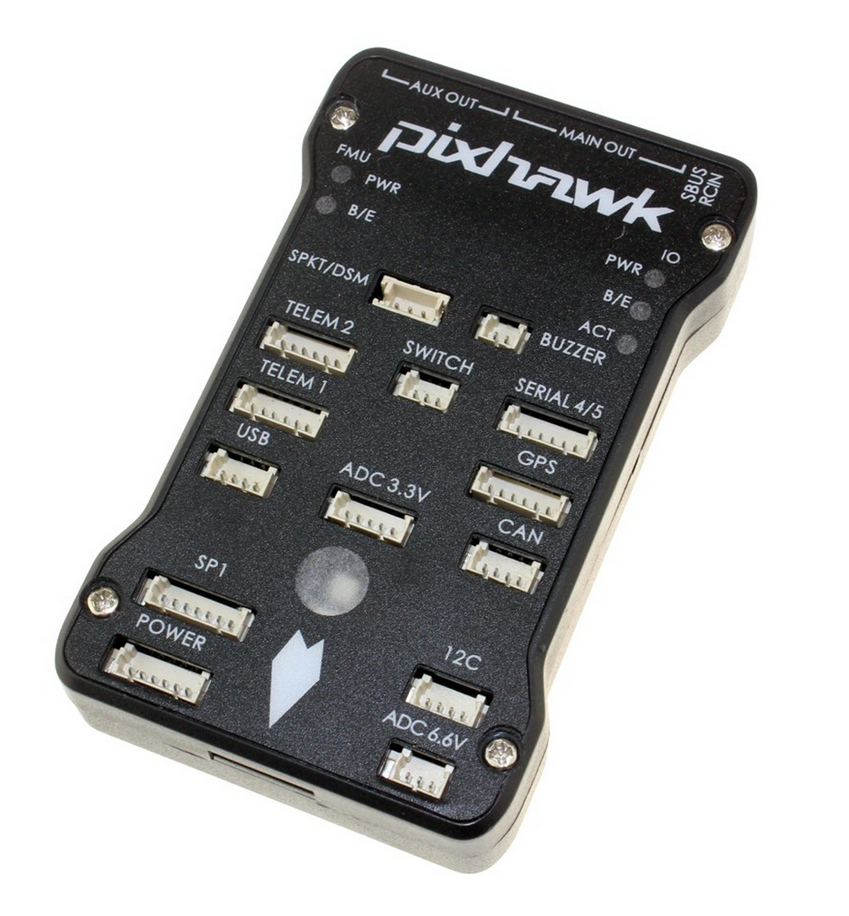
\includegraphics[height=7cm]{imagenes/cap3/7_px4_logo.png}
	\end{center}
	\caption[Controlador PX4]{Controlador PX4}
	\label{fig:px4autopilot}
\end{figure}

\section{Iris}
\label{sec:iris}

Es el nombre de la aeronave usada para solucionar los problemas planteados. En síntesis, es un dron cuadracóptero provisto de una cámara y un sensor de \ac{RF} simulado. Dicha aeronave es cortesía de \textbf{JdeRobot}, que es una organización sin ánimo de lucro, asociada a \emph{RoboticsLabURJC}, que provee de un conjunto de herramientas pensadas para desarrollar aplicaciones robóticas \footnote[16]{\url{https://jderobot.github.io/}}.\\

\begin{figure} [H]
	\begin{center}
	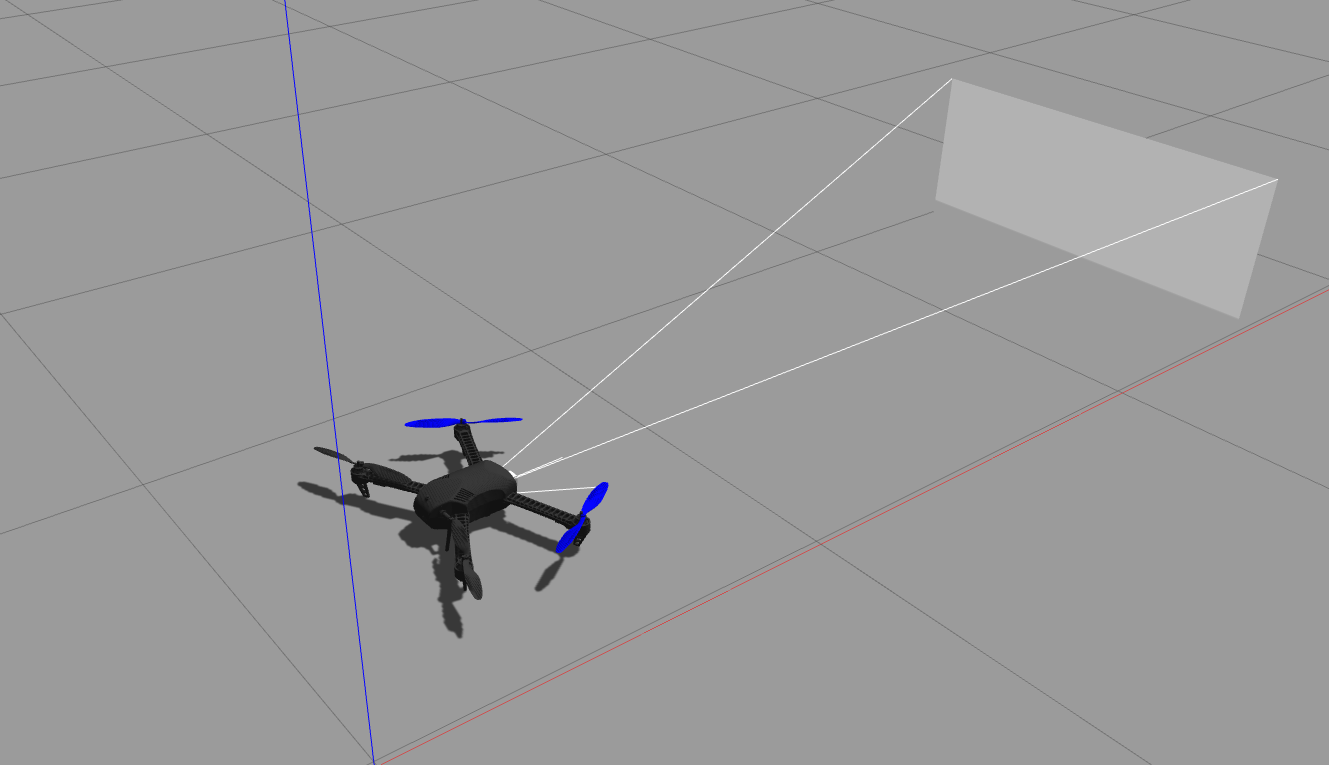
\includegraphics[height=5cm]{imagenes/cap3/8_iris_drone.png}
	\end{center}
	\caption[Iris drone en Gazebo 11]{Iris drone en Gazebo 11}
	\label{fig:irisdrone}
\end{figure}